
% This LaTeX was auto-generated from MATLAB code.
% To make changes, update the MATLAB code and republish this document.

\documentclass{article}
\usepackage{graphicx}
\usepackage{color}

\sloppy
\definecolor{lightgray}{gray}{0.5}
\setlength{\parindent}{0pt}

\begin{document}

    
    
\section*{main.m}


\subsection*{Contents}

\begin{itemize}
\setlength{\itemsep}{-1ex}
   \item Definitions
   \item Part (a)
   \item Part (b)
   \item Part (c)
   \item Part (d)
\end{itemize}


\subsection*{Definitions}

\begin{verbatim}
func = @(x) 2./(exp(x) - 1) - 2./sqrt(x) + 1;
dfunc = @(x) 1./x.^(3/2) - 2*exp(x)./(exp(x) - 1).^2;
\end{verbatim}


\subsection*{Part (a)}

\begin{verbatim}
a = func([0.5, 1.7, 2.1, 4.5])
\end{verbatim}

        \color{lightgray} \begin{verbatim}
a =

    1.2546   -0.0869   -0.1010    0.0797

\end{verbatim} \color{black}
    

\subsection*{Part (b)}

\begin{verbatim}
b = dfunc([0.5, 1.7, 2.1, 4.5])
\end{verbatim}

        \color{lightgray} \begin{verbatim}
b =

   -5.0070   -0.0958    0.0106    0.0820

\end{verbatim} \color{black}
    

\subsection*{Part (c)}

\begin{verbatim}
subplot(2, 1, 1)
xs = linspace(0, 100, 500);
plot(xs, func(xs))

subplot(2, 1, 2)
xs = linspace(1/2, 10, 500);
plot(xs, func(xs))
\end{verbatim}

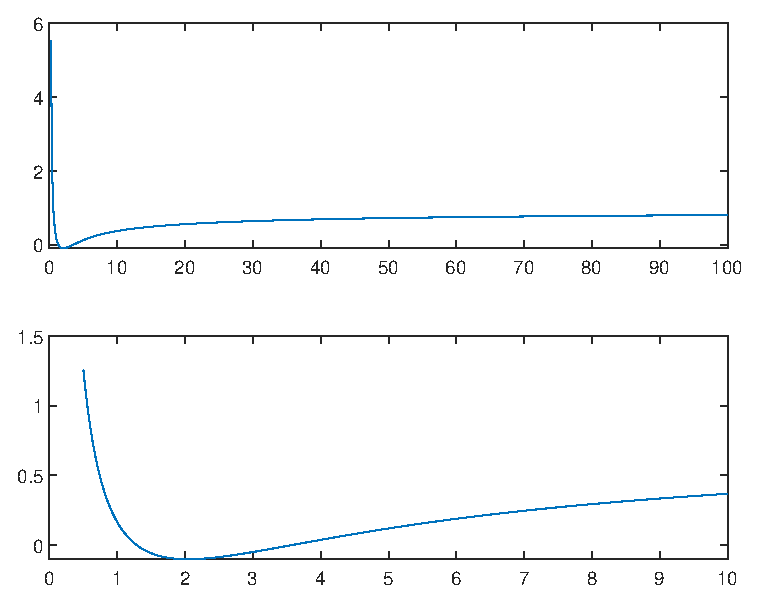
\includegraphics [width=4in]{main_01.eps}


\subsection*{Part (d)}

\begin{verbatim}
tol = 1e-6;
for i=1:10
	str = sprintf('Init. val: %d', i);
	disp(str)
	disp(newton(func, dfunc, i, tol));
end
\end{verbatim}

        \color{lightgray} \begin{verbatim}Init. val: 1
    1.2866

Init. val: 2
No convergence
Init. val: 3
    3.5764

Init. val: 4
    3.5764

Init. val: 5
    3.5764

Init. val: 6
    3.5764

Init. val: 7
    3.5764

Init. val: 8
    1.2866

Init. val: 9
No convergence
Init. val: 10
No convergence
\end{verbatim} \color{black}
    


\end{document}

